Общая блок-схема устройства представлена на рисунке~\ref{fig:commonscheme}.

\begin{figure}[ht]
    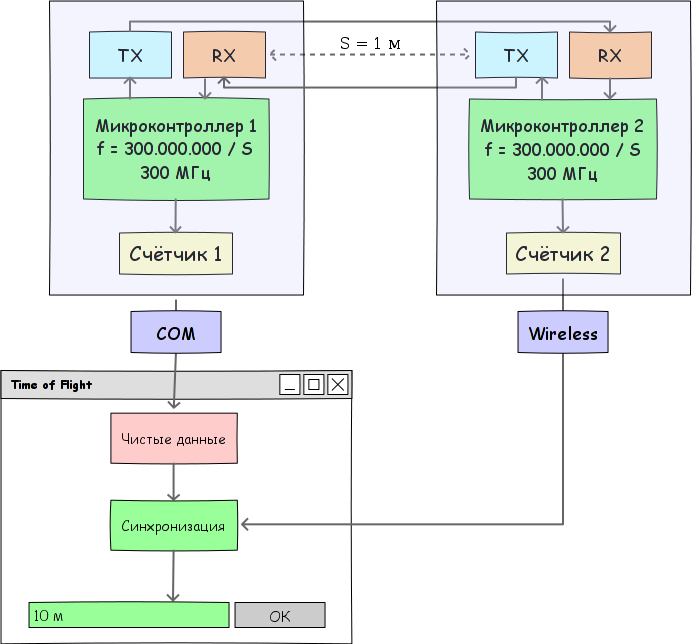
\includegraphics[width=1\linewidth]{Figures/commonscheme.png}
    \caption{Общая блок-схема Time of Flight устройства}
    \label{fig:commonscheme}
\end{figure}

Здесь модуль 1 соединён с ЭВМ посредством COM-порта, когда модуль 2 общается с модулем 1 лишь посредством радиосвязи. После завершения рассчёта времени Time of Flight, модуль 2 посылает данные, измеренные с помощью локального тактового генератора, на модуль 1 посредством радиосвязи, после чего модуль 1, пользуясь <<полной картиной>>, посылает данные на ЭВМ через последовательный порт.

Скорость общения по COM-порту была выбрана в 115200 бит/c.

Схема подключения оборудования одного модуля представлена на рисунке~\ref{fig:circscheme}.

\begin{figure}[ht]
    \subfloat[]{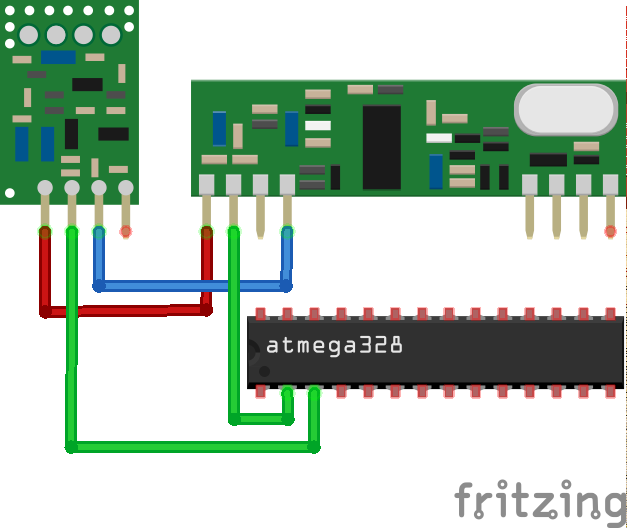
\includegraphics[width=.3\linewidth]{Figures/hardscheme.png}}
    \qquad
    \subfloat[]{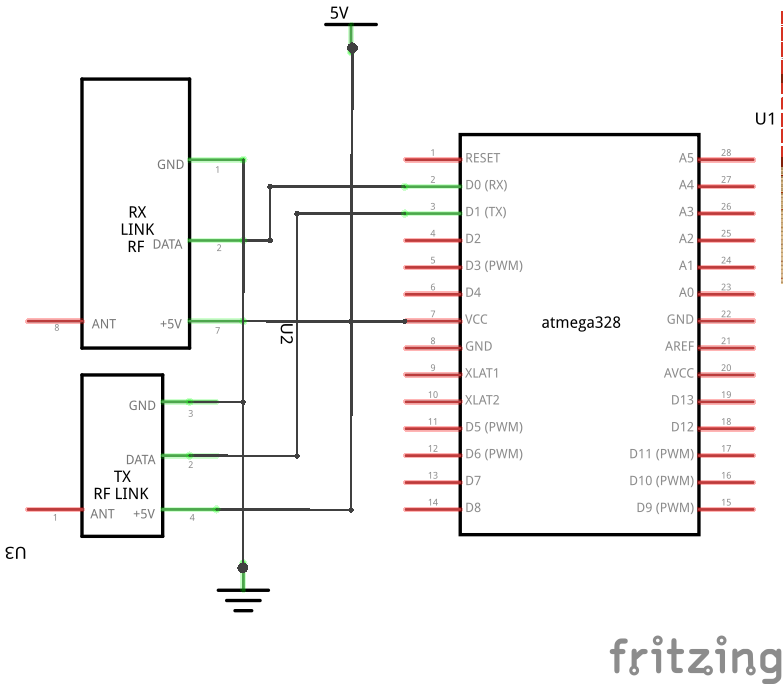
\includegraphics[width=.6\linewidth]{Figures/circscheme.png}}
    \caption{Подключение оборудования (а) общий вид; (б) схемотехника}
    \label{fig:circscheme}
\end{figure}

Здесь к микроконтроллерному модулю подключены передатчик и приёмник, работающие на несущей частоте 433 МГц и общающиеся непосредственно с другим модулем. Схема другого модуля будет выглядеть точно также, отличаться будет лишь исходный код программы.
